\documentclass[12pt]{article}
\usepackage[utf8]{inputenc}
\usepackage{upquote}
\usepackage[margin=1in]{geometry} 
\usepackage{amsmath,amsthm,amssymb}
\usepackage{graphicx}
\usepackage{listings}
\newenvironment{statement}[2][Statement]{\begin{trivlist}
\item[\hskip \labelsep {\bfseries #1}\hskip \labelsep {\bfseries #2.}]}{\end{trivlist}}
\usepackage{xcolor}

\usepackage{booktabs}
\usepackage{subfigure}


% Listings package for code rendering (No external dependencies)
\usepackage{listings}  
\usepackage{xcolor}   % Color support
\usepackage{tcolorbox} % Box for better appearance

% Define custom colors for code highlighting
\definecolor{codegreen}{rgb}{0,0.6,0}
\definecolor{codegray}{rgb}{0.5,0.5,0.5}
\definecolor{codepurple}{rgb}{0.58,0,0.82}
\definecolor{backcolour}{rgb}{0.95,0.95,0.92}


\lstset{frame=tb,
    language=Python,
    backgroundcolor=\color{backcolour},   
    commentstyle=\color{codegreen},
    keywordstyle=\color{magenta},
    numberstyle=\tiny\color{codegray},
    stringstyle=\color{codepurple},
    basicstyle=\ttfamily\footnotesize,
    breakatwhitespace=false,         
    breaklines=true,                 
    keepspaces=true,                 
    numbers=left,       
    numbersep=5pt,                  
    showspaces=false,                
    showstringspaces=false,
    showtabs=false,                  
    tabsize=2,
}

\title{Handin 3}

\begin{document}
\maketitle

\section{Introduction}

%Outlines the report.
%Contains information about contents, (research) questions and overall structure.

We evaluates the Conjugate Gradient (CG) and Approximate Newton algorithms for optimization on $f_1$, $f_4$, and $f_5$. Key objectives include:
\begin{itemize}
    \item Performance analysis under different $\eta$ schedules
    \item CG step efficiency analysis
    \item Comparison of the original Newton's algorithm and Steepest Descent to approximate Newton
\end{itemize}


\section{Theory Questions}
\subsection{Question 1.1}

From equation (20), we have:
\[
p_{k+1} = v_{k+1} - \sum_{i=0}^{k} \beta_i p_i.
\]
Since $v_{k+1} = -\nabla f(x_{k+1})$, this can be rewritten as:
\[
p_{k+1} = -\nabla f(x_{k+1}) + \sum_{i=0}^{k} \beta_i p_i.
\]
By induction, the gradient at any step $k$ can be expressed as a linear combination of the search directions:
\[
\nabla f(x_k) = \sum_{i=0}^{k} \gamma_i p_i,
\]
for some coefficients $\gamma_i$, proving the desired result.

\subsection{Question 1.2}

From Theorem 6, we know that for a quadratic function:
\[
\nabla f(x_{k+1})^T p_i = 0, \quad \forall i \leq k.
\]
Since $p_i$ are conjugate with respect to $Q$, we express each gradient as:
\[
\nabla f(x_k) = \sum_{i=0}^{k} \gamma_i p_i.
\]
Taking the dot product with $\nabla f(x_j)$ for $j < k$:
\[
\nabla f(x_k)^T \nabla f(x_j) = \left( \sum_{i=0}^{k} \gamma_i p_i \right)^T \nabla f(x_j).
\]
By the conjugacy property, each $\nabla f(x_j)$ is a linear combination of $p_0, \dots, p_j$, and:
\[
\nabla f(x_k)^T \nabla f(x_j) = 0.
\]
Thus, the gradients remain mutually orthogonal.


\subsection{Question 2}

Using equation (21):
\[
p_{k+1} = -\nabla f(x_{k+1}) + \sum_{i=0}^{k} \beta_i p_i.
\]
Since each $p_i$ is a linear combination of past gradients, we conclude that:
\[
p_i \in \text{span}\{ \nabla f(x_0), \dots, \nabla f(x_i) \}.
\]
Thus, every search direction lies within the Krylov subspace:
\[
\mathcal{K}_k(Q, \nabla f(x_0)) = \text{span}\{ \nabla f(x_0), Q \nabla f(x_0), \dots, Q^k \nabla f(x_0) \}.
\]
This confirms the result.

\section{Experiments}

\subsection{Implementation Correctness Validation}

To ensure the correctness of the Approximate Newton, we check the following pointsin our code.

\begin{itemize}
    \item Check Positive Definiteness Validation by using $np.linalg.cholesky(H)$:
\begin{lstlisting}
def is_positive_definite(H):
    try:
        np.linalg.cholesky(H)
        return True
    except np.linalg.LinAlgError:
        return False
\end{lstlisting}
    \item Ensure different $\eta_k$ to expected theoretical convergence:
\begin{lstlisting}
        if eta_type == "linear":
            eta_k = 1/2 
        elif eta_type == "superlinear":
            eta_k = 1/2 * min(1/2, sqrt(norm_g))
        elif eta_type == "quadratic":
            eta_k = 1/2 * min(1/2, norm_g)
        else:
            raise ValueError("Invalid eta_type.")
\end{lstlisting}
    \item Implement CG stopping criteria to ensure correct termination:
\begin{lstlisting}
eps_k = eta_k * norm_g
\end{lstlisting}
\end{itemize}

\subsection{Parameter Settings}
\begin{tabular}{ll}
    \toprule
    Parameter & Values \\ 
    \midrule
    $x_0$ &  Sample from the standard normal distribution (mean=0, stdev=1).\\
    $\eta$ schedules & Linear ($\eta_k = 1/2$), Superlinear, Quadratic \\
    Stopping criteria & $\|\nabla f\| < 10^{-6}$ \\
    Max iterations & 15 \\
    \bottomrule
\end{tabular}

\subsection{Function Selection}
We exclude $f_2$, $f_3$ in our experiment. 

The Hessian of $f_1$ is $2*diag(w)$ where $w$ contains strictly positive values. It is always positive definite since all diagonal entries are positive.

The Hessian of $f_2$ has negative term like $x=(0,2)$, and the Hessian here is $[[-798, 0], [0, 200]]$. The leading principal minor is negative, so the matrix is indefinite. 

The Hessian of $f_3$ can have negative eigenvalues from $np.outer(g,g)$. For example when $x=[0.1,0]$, the Hessian is not positive semi-definite.

The Hessian of $f_4$ is always positive definite, because $h(x,q)$ and its derivatives are non-negative in diagonal entries.

The Hessian of $f_5$ is always positive definite, because the diagonal term is $factor*(factor-1)*|x_i|^{factor-2}$, which is non-negative.


\section{Results and Discussion}

\subsection{Convergence Behavior and Analysis}

Performance of approximate Newton algorithm under different schedules of $\eta_k$ is as shown in figure ~\ref{fig:convgraph}. We can see the Quadratic  convergences fastest, then the Superlinear, and the Linear Convergence the slowest. 

It is clear in $f_1$ and $f_4$ that the quadric schedule can achieve a Quadratic Convergence, and the error decreases sharply, forming an "L"-shaped curve in the last stage. The superlinear schedule can achieve a Superlinear Convergence, and the rate of decrease accelerates progressively, with the curve becoming steeper over time. The linear schedule can achieve a Linear Convergence, Exhibiting a straight-line decline on a logarithmic plot, with a constant slope.

But for $f_5$ all the three strategies performs as linear convergence, which is quite surprising. We analyze the reason as follows:

For the Hessian of $f_5$, the diagonal elements corresponding to each variable are given by:
\[
\text{Hessian}_{ii} = \text{factor} \cdot (\text{factor} - 1) \cdot |x_i|^{\text{factor} - 2}.
\]
Here, the \textit{factor} increases linearly; for example, in the two-dimensional case, the factors are 2 and 4. As $x_i$ approaches zero, the Hessian element for the term with $\text{factor} = 2$ simplifies to:
\[
2 \cdot (2-1) \cdot |x_i|^0 = 2,
\]
while for $\text{factor} = 4$, it becomes:
\[
4 \cdot 3 \cdot |x_i|^2.
\]
As $x$ approaches zero, the Hessian elements of the higher-order terms tend to zero, which may cause the Hessian matrix to become very small in certain variable directions. Consequently, this may result in the Hessian matrix being nearly positive semi-definite but with a poor condition number. So the approximate Newton will not perform well.


\begin{figure}[ht]
\centering
\subfigure[Ellipsoid function($f_1$)]{
    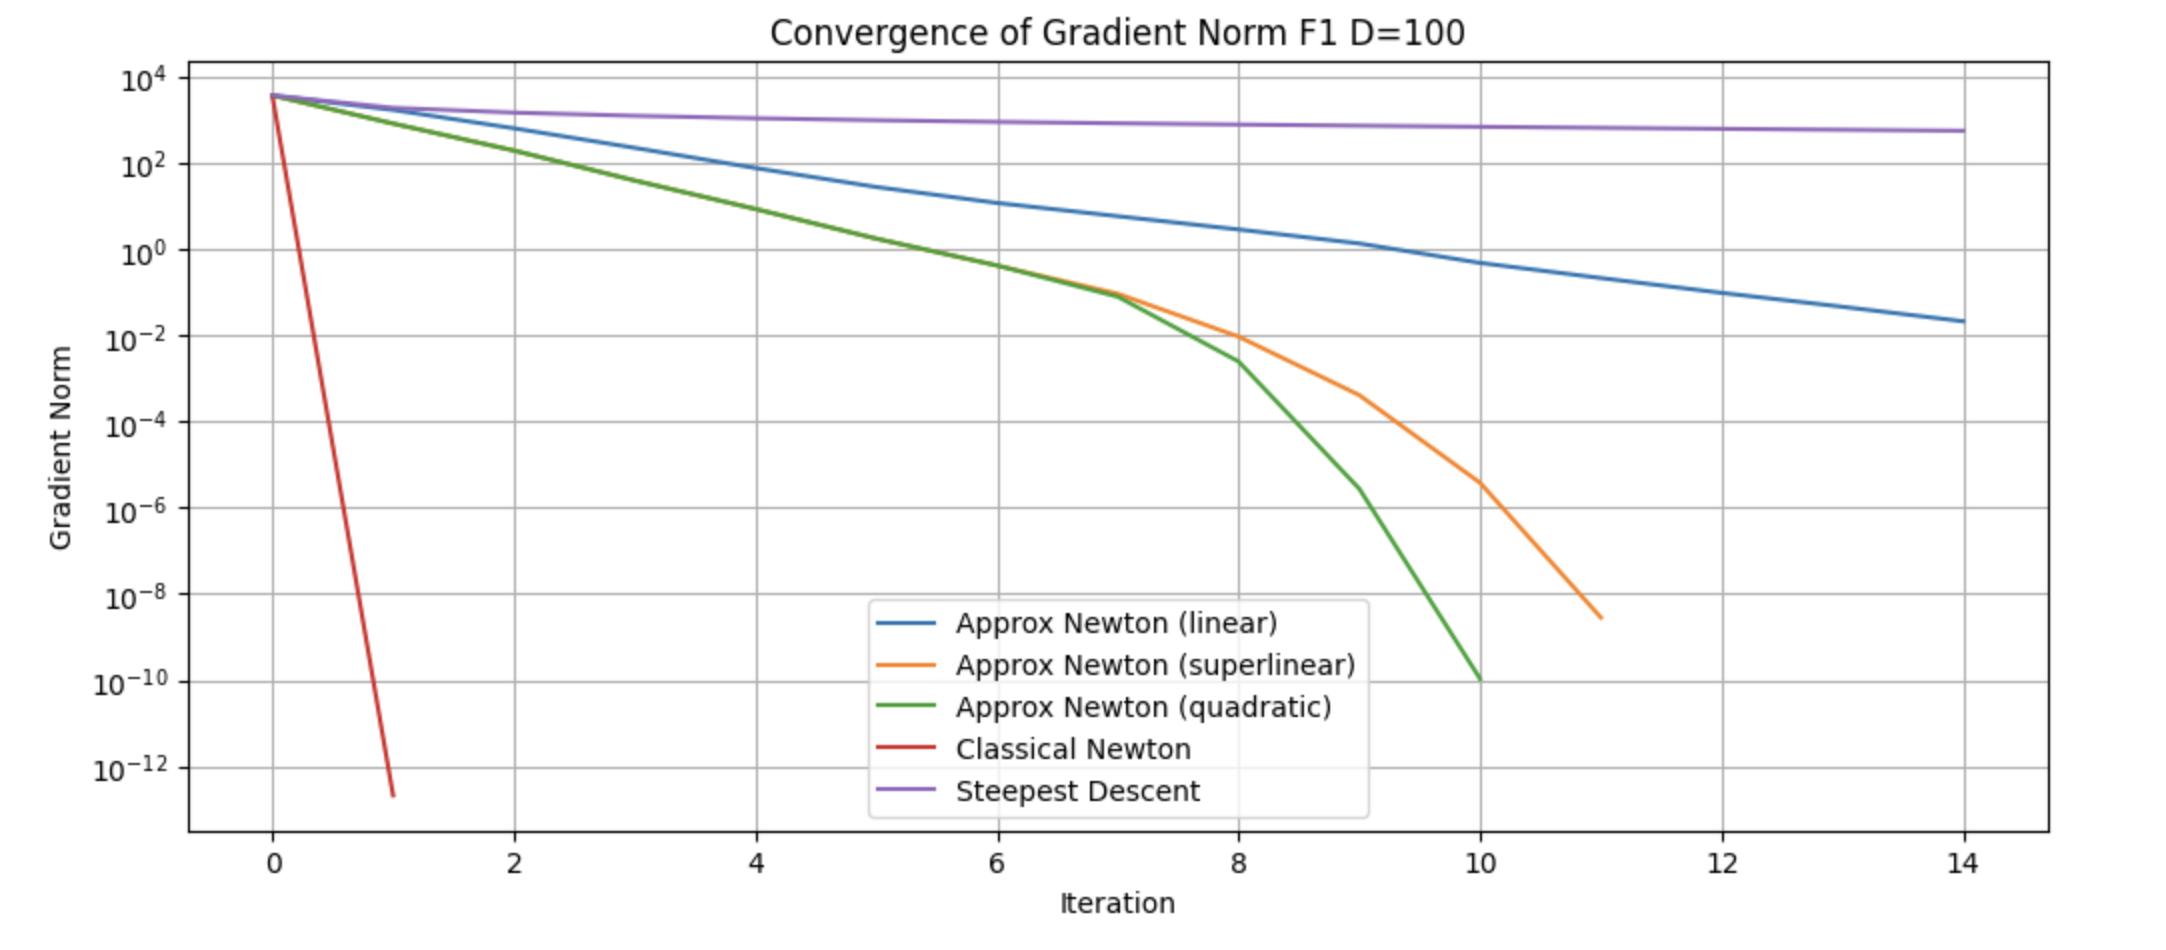
\includegraphics[width=0.3\columnwidth, keepaspectratio]{pics/h3-1}
\label{fig:f1}
}
\subfigure[Attractive-Sector Function($f_4$)]{
    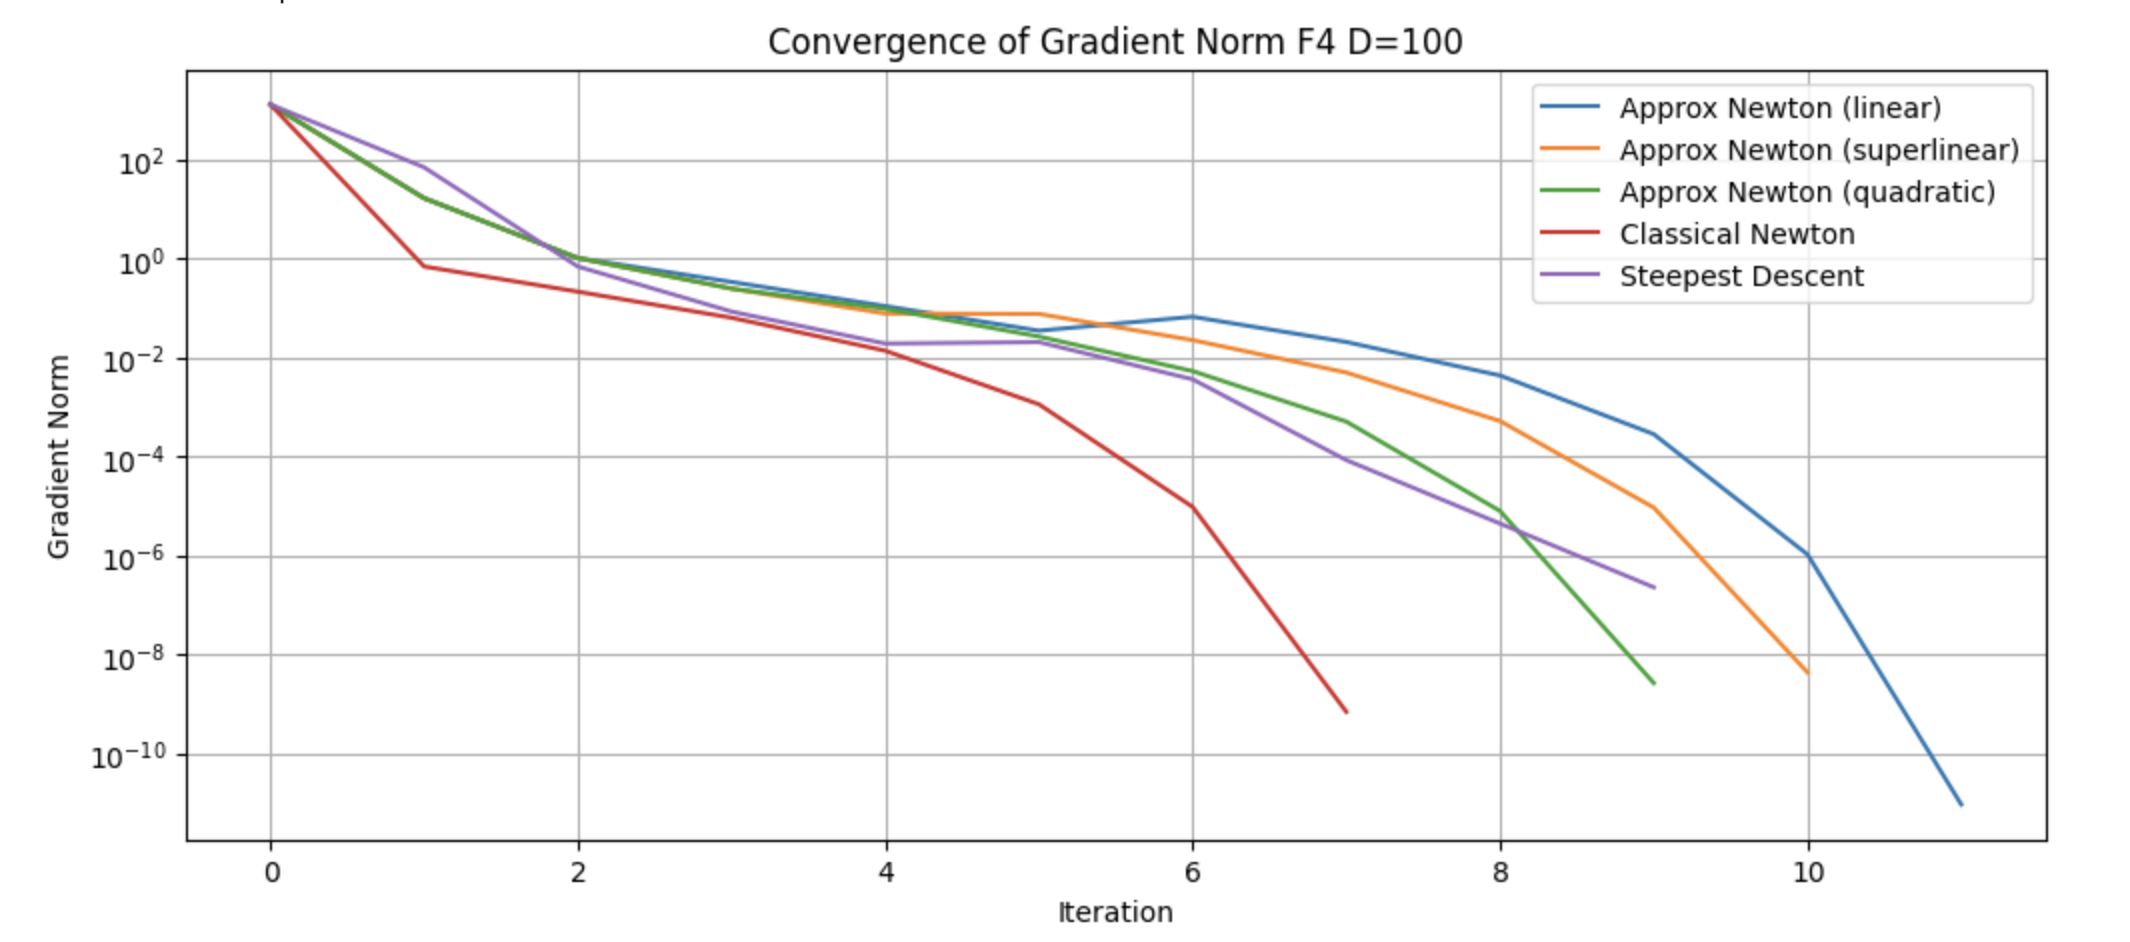
\includegraphics[width=0.3\columnwidth, keepaspectratio]{pics/h3-4}
    \label{fig:f4}
}
\subfigure[Sum of Different Powers Function($f_5$)]{
    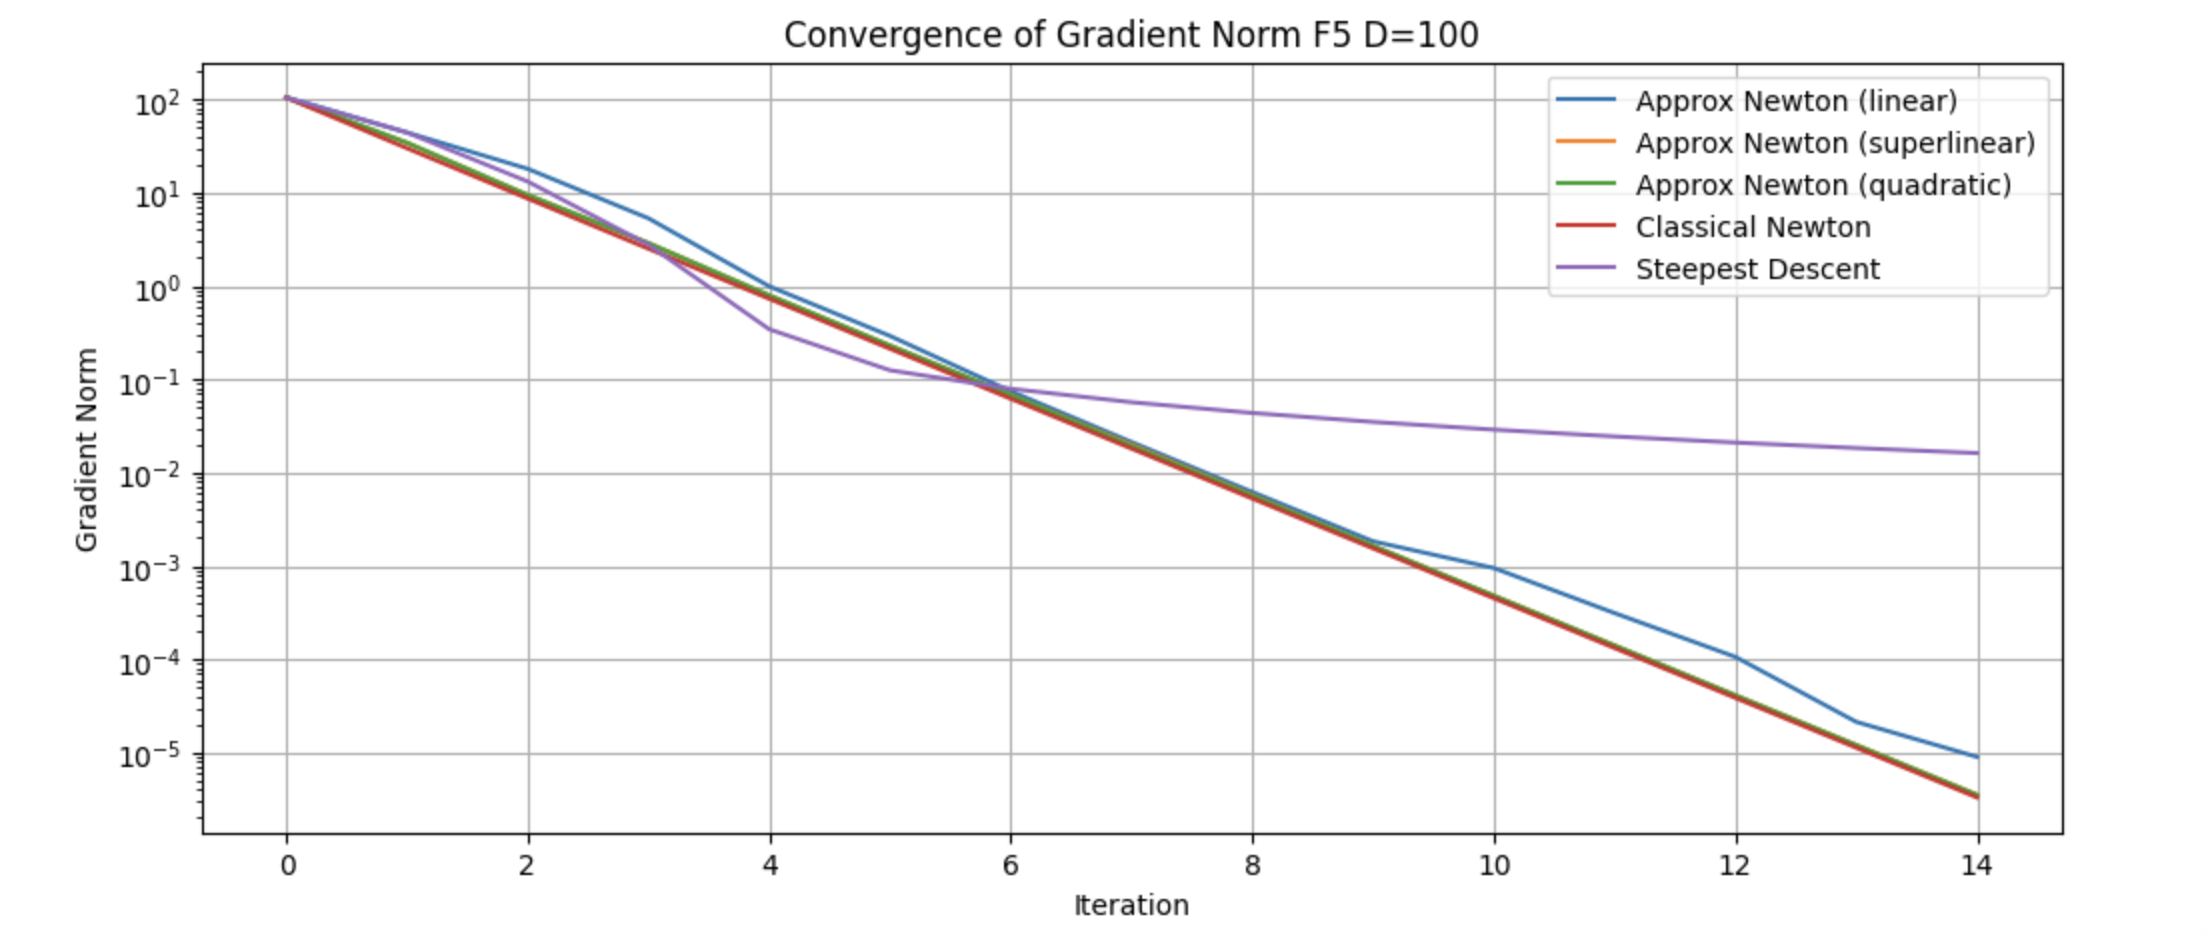
\includegraphics[width=0.3\columnwidth, keepaspectratio]{pics/h3-5}
    \label{fig:f5}
}
\caption[]{Comparison of convergence rates under different $\eta$ schedules with $f_1$, $f_4$, $f_5$}
\label{fig:convgraph}
\end{figure}

\subsection{CG Step Efficiency}
Due to page limitation we only evaluate $f_1$ here. Our observations are as follows:

\begin{itemize}
    \item Linear Approximate Newton uses fewer CG steps per iteration (~7.87), and trades accuracy per iteration for more iterations overall.
    \item Quadratic Convergence: there needs to be more CG iterations per step.
    \item Superlinear Convergence: Faster than linear but not as fast as quadratic.
\end{itemize}

% TODO Superlinear convergence requires careful $\eta$ scheduling.

\begin{table}[h]
    \centering
    \begin{tabular}{lccc}
        \toprule
        \textbf{$\eta_k$ Schedule} & \textbf{Iterations} & \textbf{Total CG Steps} & \textbf{CG Steps per Iteration} \\
        \midrule
        Linear & 15 & 118 & 7.87 \\
        Superlinear & 11 & 142 & 12.91 \\
        Quadratic & 10 & 130 & 13.00 \\
        \bottomrule
    \end{tabular}
    \caption{CG Step Analysis for Different $\eta_k$ Schedule in Approx. Newton with $f_1$}
    \label{tab:cg_steps}
\end{table}

\subsection{Method Comparison}
We also plot the convergence graph of classic newton and steepest descent in Figure ~\ref{fig:convgraph}. The computational cost refers to the complexity of calculating the Hessian, both time and memory.

Classic Newton performs well when the Hessian Matrix is positive definite, and when its easy to calculate, the time and memory cost can be controlled. The Steepest Descent performs the worst but with low computational cost. The approximate newton method is a middle choice between them. So if the Hessian is positive definite, we prefer to choose Approximate Newton for a trade off of resources and efficiency; else we will use Steepest Descent.

\section{Conclusion}

We find Classical Newton performs well for the problem with cheap Hessians($f_1$), and generally approximate Newton provides best balance for $d \geq 100$ ($f_4$, $f_5$). We can adapt $\eta$ schedules for a more optimal performance.


\end{document}
